\documentclass[a4paper,12pt]{article}
\usepackage{graphicx}
\usepackage[UTF8]{ctex}
\usepackage{fontspec}
\usepackage{booktabs}
\usepackage{float}%浮动体
\usepackage{amsmath,amssymb}
\usepackage{fancyhdr}
%\usepackage{xcolor}
\usepackage{colortbl}
\usepackage{geometry}
\geometry{top=2cm,bottom=2cm,left=1cm,right=1cm}
\begin{document}
	\begin{figure}[H]
	\begin{center}
		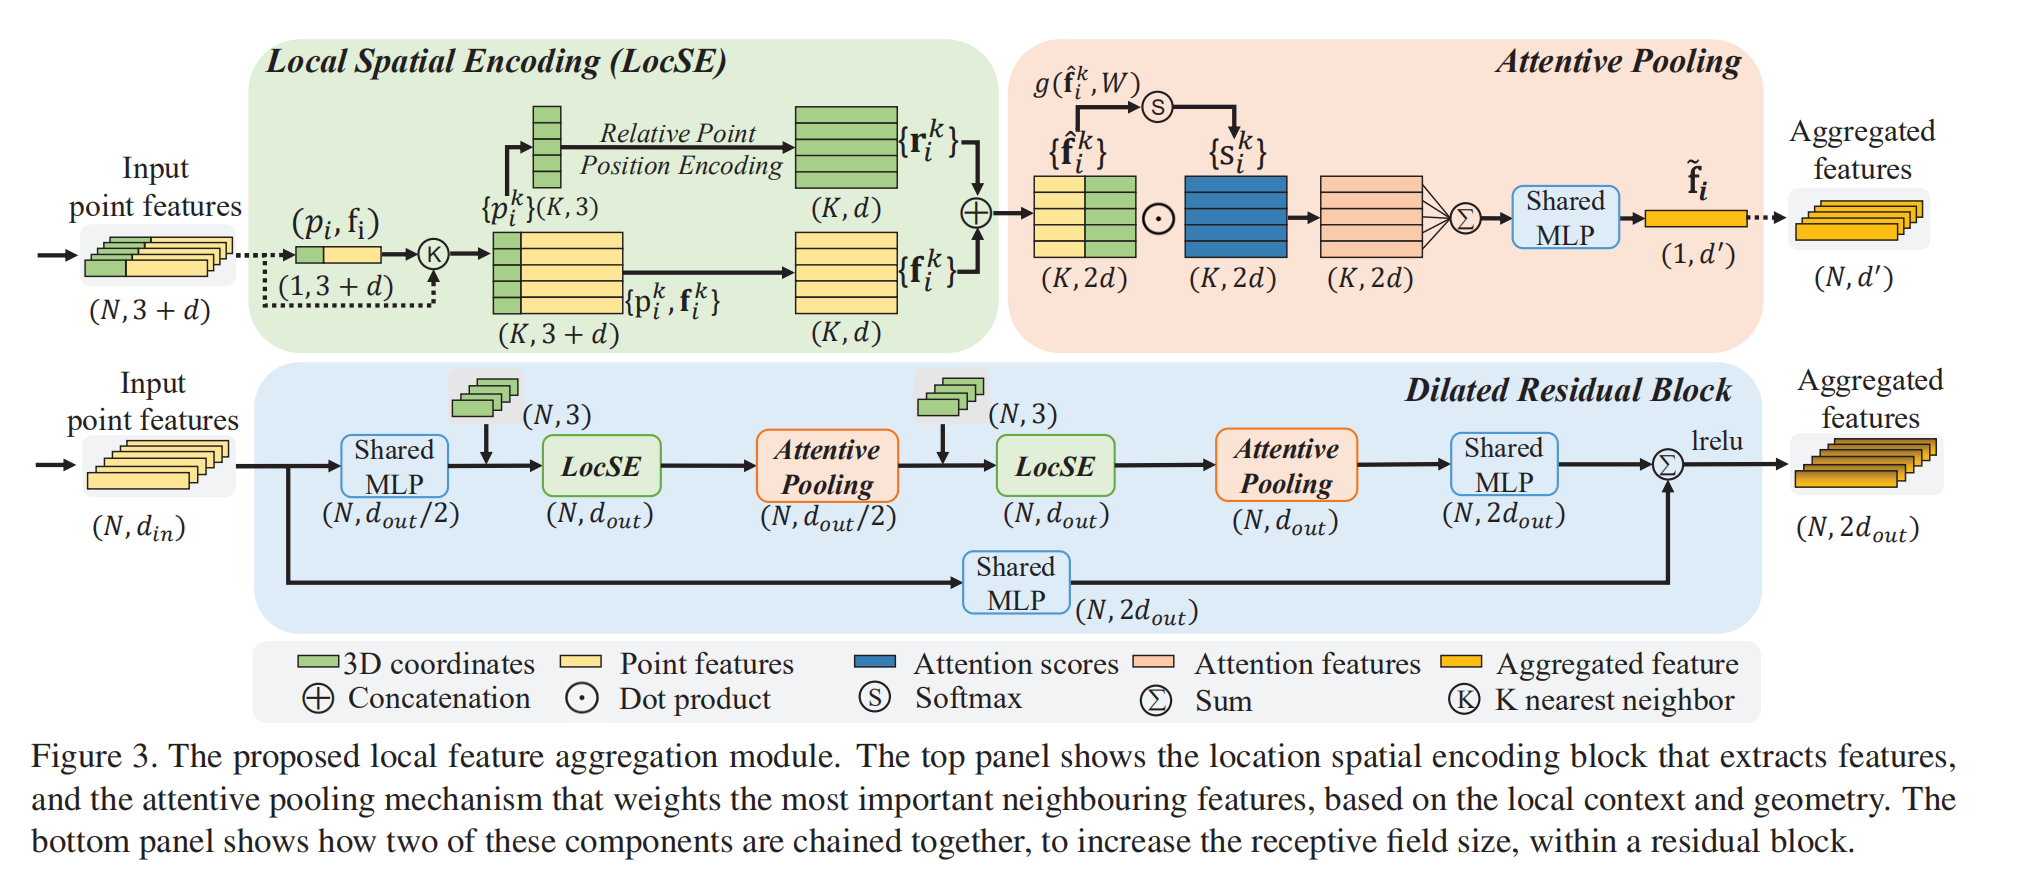
\includegraphics[width=0.9\textwidth]{img/RandLA_Net.png} 
		\caption{RandLA\_Net}
	\end{center}
\end{figure}


\textbf{分析}:
\begin{itemize}
	\item 随机采样,然后通过local spatial encoding, Attentive Pooling通过类似ResNet的结构组织起来,对特征进行聚合。(能够处理较大规模的数据)
	\item 
\end{itemize}
	$$
\mathbf{r}_{i}^{k}=M L P\left(p_{i} \oplus p_{i}^{k} \oplus\left(p_{i}-p_{i}^{k}\right) \oplus\left\|p_{i}-p_{i}^{k}\right\|\right)
$$


\paragraph{语义分割} 通过叠加4个局部特征聚合模型,对点云的特征进行编码(encoder),然后使用MLP对聚合的特征进行decoder,最后对每个点进行分类(mlp)

\end{document}